\documentclass[submit,techreq,noauthor]{eco}	% semi style
\usepackage[dvips]{graphicx}
\usepackage{listings, jlisting} 		% for source code
\usepackage{url}
\usepackage{setspace}
\usepackage{here}
%\setstretch{1.5} % 行間を広くします(資料チェックしてもらうときはコメントを外す)
\lstset{
  basicstyle={\ttfamily},
  identifierstyle={\small},
  commentstyle={\smallitshape},
  keywordstyle={\small\bfseries},
  ndkeywordstyle={\small},
  stringstyle={\small\ttfamily},
  frame={tb},
  breaklines=true,
  columns=[l]{fullflexible},
  numbers=left,
  xrightmargin=0zw,
  xleftmargin=3zw,
  numberstyle={\scriptsize},
  stepnumber=1,
  numbersep=1zw,
  lineskip=-0.5ex
}

\begin{document}

\semino {4/7}					% 年度/回数
\date   {4/11/25/金}				% 平成/月/日/曜日
\title  {Operating System Support for Safe and Efficient Auxiliary Execution}	% タイトル
\author {山下 恭平}				% 氏名

\begin{abstract}
本稿はUSENIX,OSDI'22 に掲載されている論文「Operating System Support
 for Safe and Efficient Auxiliary Execution」\begin{math}^{[1]}\end{math}の内容についてまとめた
ものである.近年のアプリケーションは様々な補助タスクが実行されている.補助タスクとは,アプリ
ケーションが自身のメンテナンス,自己管理を行うタスクのことである.これらのタス
クは、アプリケーションのアドレス空間で実行することで,高い観測性と制御性
を得るが,安全性と性能の問題が発生する.また,補助タスクを別のプロセスで実行す
ると,分離性は高いが,観測性と制御性が劣る.本稿では,この問題を解決するために,
補助タスクに対するサポートとして,orbitと呼ばれるOSの抽象化機能を提案する.

\end{abstract}
\maketitle

\section{はじめに}
運用されているアプリケーションはその実行状況を調査し,最適化し,デバッグし,
制御するために,頻繁にメンテナンスを行う必要がある.かつてはメンテナンスはアプリケ
ーションの管理者が手動で行なっていたが,現在では多くのアプリケーションは,自身
でメンテナンスを行うための補助タスクが行われている.例えばMySQLでは,デッド
ロックを検出するとロールバックを行う機能が存在する.\begin{math}^{[2]}\end{math}
そのため補助タスクはアプリケーションの信頼性や観測性に大きく影響する.
\indent 既存のOSに搭載されているプロセスやスレッドといった抽象化機能は
メインタスクの実行に適した設計がされており,補助タスクの実行には適していない.
そのため,開発者は,分離は強いが観測と制御が非常に限定される(別プロセス)か,
観測と制御は強いが分離はほとんどできない(スレッド)かのどちらかを選ばざる
を得ない.この問題を解決するために,OSの補助タスクに対するサポートを提供する
orbit抽象化を提案する.\\
\indent orbitタスクは,協力な分離を提供する.同時に,状態同期機能により
メインタスクを観測することも可能である.orbitのプロトタイプはLinux kernel 
5.4.91に実装された.orbitの評価を行うためにMySQL,Apacheを含む6つの大規模
アプリケーションから,7つの補助タスクを抽出し,orbitに移行することに成功した.
また,全てのケースでアプリケーションはフォールトから保護されることがわかった.
分離のコストを測定した所.orbitバージョンアプリケーションでは,中央値で3.3
\%のオーバーヘッドが発生した.\\
\indent 本稿では2章でこの研究が行われる背景について述べ,3章でorbitの詳細な
説明を行う,4章でorbitの性能評価を行い,最後の5章では全体のまとめる.

\section{研究の背景}

\begin{figure}[H]
  \centering
  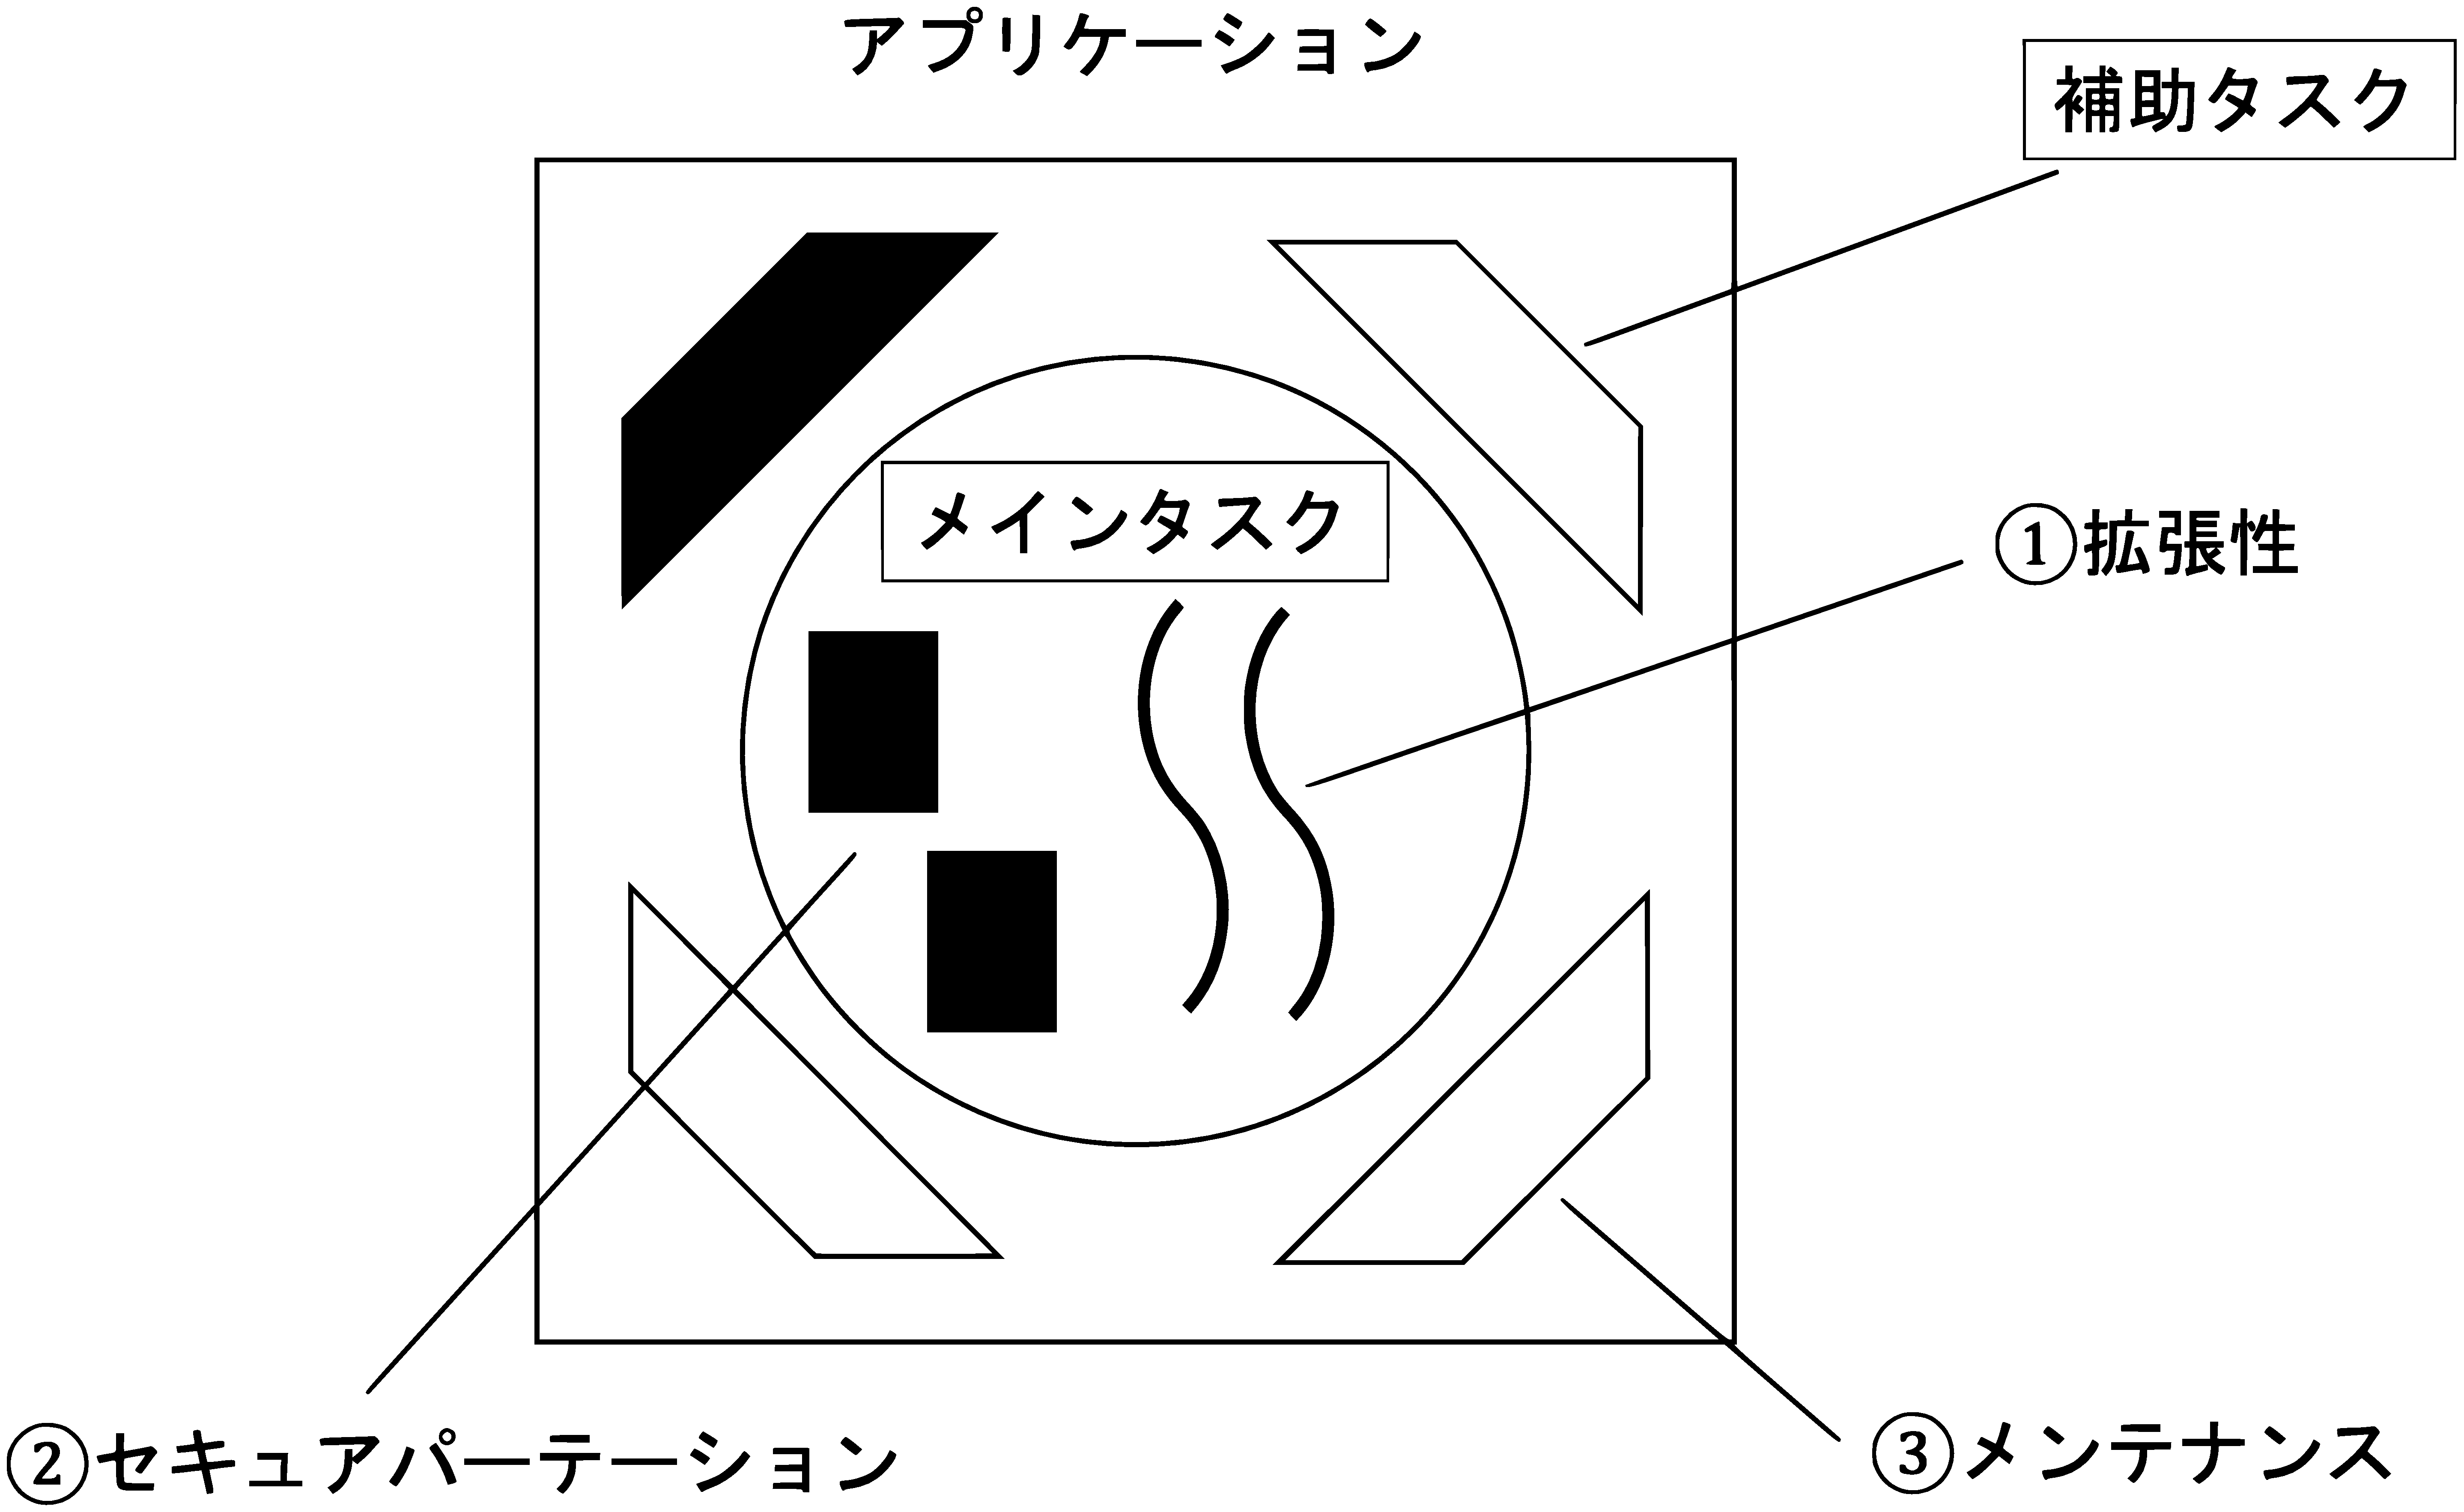
\includegraphics[width=5.5cm]{fig/pic1.eps}
  \caption{アプリケーション構成}
\end{figure}

アプリケーションはメインタスクと補助タスクの2つの論理領域に分けることができる.
図1はアプリケーションの構成を示したものであり,メインタスクの周辺に補助タスクが
存在することがわかる.(1)から(3)については後から説明を行う.補助タスクはメインタスク
のサポートを行うために,、メインタスクを観測し,制御する必要がある.この時,補助タスク
のバグによってがメインタスクに影響が出ないようにするため,メインタスクと補助タスクの
隔離を行う必要がある.つまり,補助タスクには,観測性,制御性,隔離が必要である.

\subsection{タスクの実行方法}
\indent 既存のOSでは補助タスクは主に2種類の実行方法をとる.
1つ目は,メインプログラムと同一のアドレス空間に配置され,メインタスクの関数,
スレッドとして実行される方法だ.この方法であれば,補助タスクはメインタスクの観測,制御が
容易に行うことができる.しかし,補助タスクによってメインタスクが不必要なブロックが起こる
可能性や,補助タスクにバグが存在した場合,メインタスクにまで影響が出るため,隔離について不十分
である.
2つ目はメインタスクと補助タスクを別プロセスで実行する方法だ.この方法であれば,
メインタスクと補助タスクは異なるアドレス空間に存在するため,隔離が十分に行えている.しかし,
メインタスクの観測と制御が困難になる.プロセスやスレッドといった機能は1章で述べた通り,
補助タスクの実行には適していないことがわかった.

\subsection{タスク実行の保護}
\indent タスク実行を保護するOSのサポートは既に多く研究,提案されている.しかし,それらは
異なる2つの目的のために設計されている.\\
1つはアプリケーションの拡張性のためである(図1,(1)).
具体的にはSFI\begin{math}^{[3]}\end{math}という技術がある.SFIとは,アプリケーションバイナリ
を書き換えることで,アプリケーション内の信頼できないコードのメモリアクセスを制限する
ソフトウェア隔離技術ことである.この技術はブラウザの拡張機能などの第三者が作成した
プログラムをアプリケーション内で動作させるときに有効である.\\
2つ目は,セキュアなパーテーショニングを提供するものだ(図1,(2)).具体的には
Wedge\begin{math}^{[4]}\end{math}やlwC\begin{math}^{[5]}\end{math}
といったものがある.これにより,アプリケーションが侵害された場合に,メインタスクの
機密な手続きを守ることができる.\\
しかし,これらの仕組みはアプリケーションのメンテナンス(図1,(3))にとっては不十分である.
その理由として,まず,補助タスクはアプリケーションの開発者と同一人物,機関によって開発さ
れているため,信頼できるものである.また,補助タスクはメインタスクと対話的であり,メインタス
クの状態を常に監視し,場合によっては変更を加える必要があるからだ.次の章では補助タスクの
サポートに求められるものについて述べる.

\subsection{補助タスクの安全性と性能}
1章で述べたように,メインタスクと補助タスクが同一のメモリ空間に存在する場合,補助タスクのバグに
より,無効なメモリにアクセスをした場合アプリケーション全体がクラッシュすることが考えられる.
メインタスクと補助タスクを分離した場合,補助タスクのバグによってアプリケーション全体が
クラッシュする事態は防ぐことができる.しかし,分離された補助タスクによってメインタスクの
性能が大きく低下する場合がある.MySQLのデッドロック検出タスクを実行した状態で,性能
を測定したところ,スループットが最大で79.5\%低下することが報告されている.\begin{math}^{[6]}\end{math}
このことから,補助タスクはアプリケーションの性能を維持,向上させる機能を持っているのにも関わらず,
逆にアプリケーションに害を与える可能性が存在する.\\
\indent これらの補助タスクの安全性と性能に関する懸念に対処するために,Fork-based Execution Model とS
andbox-based Execution Modelという2つの補助タスク実行モデルを紹介する.

\subsubsection*{Fork-based Execution Model}
このモデルでは,アプリケーションは補助タスクが実行される前にfork()システムコー
ルを行い,子プロセスでタスクの機能を実行するように切り替える.これにより,メインタスクと
補助タスクはアドレス空間が分離されているため,強い分離を得ることができる.また,fork()に
より,子プロセスは親プロセスのアドレス空間のコピーを保持するため,高い観測性を得られる.
しかし,子プロセスで動作が完了しても,親プロセスには変更を加えることができない,つまり,
制御性を持たないことが問題として挙げられる.また,メインタスクが大きいアドレス空間を保持
している場合,fork()によって生成される子プロセスも大きくなり,オーバーヘッドが発生する.

\subsubsection*{Sandbox-based Execution Model}
このモデルは,サンドボックス内で補助タスクを実行する方法である.サンドボックスとは,
通常使用する領域からは隔離された,保護された領域のことであり,サードパーティ製の拡張
機能などの信頼されないコードを実行するのに適している.
サンドボックス化されたプロセスは,ファイルシステムやシステムコールを含むリソース
へのアクセス権限が制限される.しかし,2.2章でも述べた通り,補助タスクは信頼できる
プログラムである.また,補助タスクにおける安全性の問題は,システムコールやファイルへの
アクセスによるものではなく,不正なメモリアクセスや無限ループなどのバグや意図しない副作用
によって発生する.さらに,サンドボックス化されたプロセスは,それらに割り当てられた
メモリセグメントのみにアクセスする.このため,メインプログラムの観測性はほとんどなく、
メインプログラムの状態を変更することもできない.

\section{orbitについて}

前章では,既存のタスク保護方法,タスク実行方法では,メンテナンスを行う
補助タスクの補助に適していないことを確認した.そこで,補助タスクの保護に
着目し,新しいOSの抽象化技法「orbit」を提案する.

\subsection{orbitの概要}
orbitには,スレッド,SFI,Wedgeなどの既存の抽象化機能と比較したとき,いくつかの
独自の特徴を持つ.
\begin{quote}
  \begin{itemize}
   \item orbitは独自のアドレス空間を保持し,スケジューリングが可能である.
   \item 各orbitはメインプロセスと結合しているが、強力に分離されている.
   \item 各orbitのアドレス空間は,メインプロセスのミラーである.
  \end{itemize}
\end{quote}
これらの特徴により,orbitタスクがクラッシュしても,メインタスクには影響は出ない.
また,orbitのアドレス空間はメインプロセスのミラーであるため,高い観測性を持つ.

\subsection{orbitの課題と解決法}
orbitの設計において大きく2つの課題が存在する.
\begin{quote}
  \begin{itemize}
   \item 分離と観測の両立が困難であること.
   \item 分離によるメインタスクの性能低下がおおきいこと.
  \end{itemize}
\end{quote}

一つ目の課題については,コピーオンライト機構を用いて,メインタスクがorbitタスクを
呼び出すたびに,メインプロセスのアドレス空間をorbitのアドレス空間へ自動的に状態
を同期させるメモリスナップショットによって解決する.

2つ目は,orbitタスクが必要とする状態だけを,orbitのアドレス空間に同期することで,
オーバーヘッドの発生を防いでいる.(図3)

\begin{figure}[H]
  \centering
  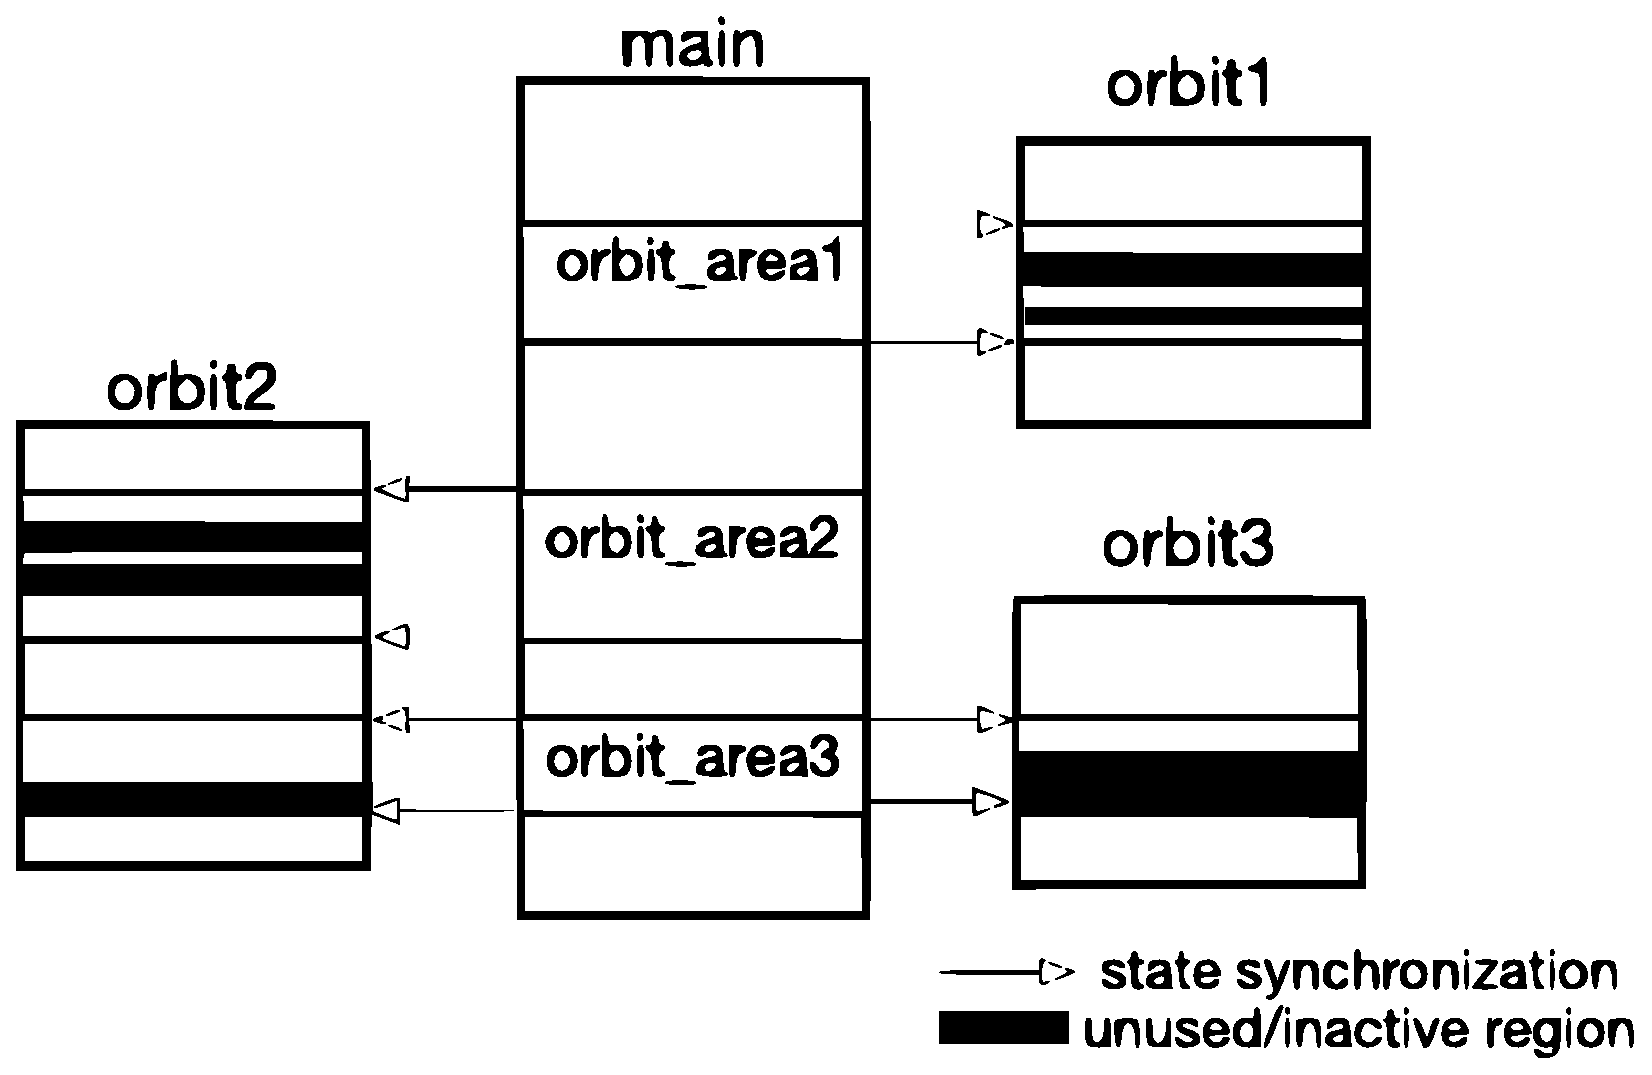
\includegraphics[width=5.5cm]{fig/pic2.eps}
  \caption{orbitタスク同期の様子}
\end{figure}

\subsection{orbitの詳細}

\begin{figure}[H]
  \centering
  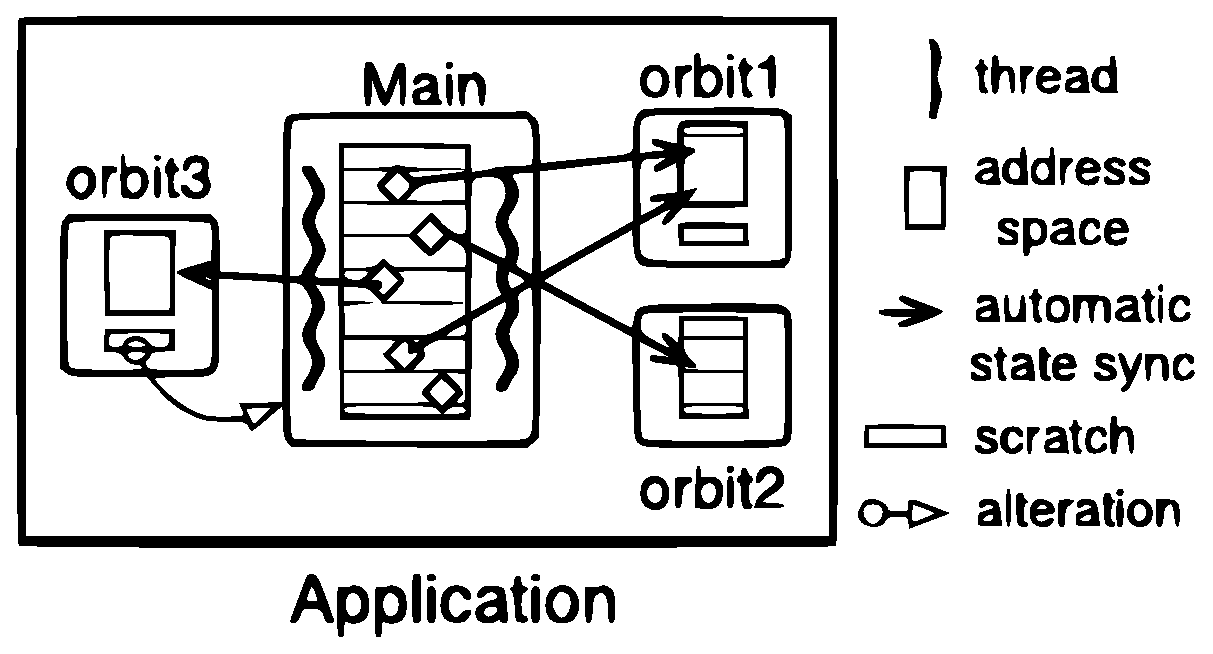
\includegraphics[width=5.5cm]{fig/pic3.eps}
  \caption{orbit動作例}
\end{figure}

orbitタスクの動作例を図3に示す,orbitの持つ特徴として,強い隔離,利便性の高いプログラミングモデル,
自動的な状態の同期,メインタスクの改変,ファーストクラスエンティティが挙げられる.ここでは,
それらの特徴について説明する.

\subsubsection*{強い隔離}
各orbitタスクにはそれぞれ独自のアドレス空間を保持する.そのため
オービット上で障害が発生しても,メインプログラムや他のオービット上のタスクが危険に
さらされることはない.また,ほとんどのオービットタスクは,メインプログラムを長時間ブロック
することなく,非同期で実行される。

\subsubsection*{利便性の高いプログラミングモデル}
orbitはAPIによって提供される.そのため,開発者はメインプログラム内にorbitタスクの
関数を書き,メインプログラムのほとんど全ての状態変数を直接参照することができる.これは
従来の開発手法であるスレッドモデルに近く,開発者が慣れ親しんだ方法で実装が可能である.
実際に,MySQLのデッドロック検出タスクは7行の追加と2行の削除で実現できた.

\subsubsection*{自動的な状態の同期}
オービットタスクのアドレス空間の特徴は,ほとんどがターゲットのアドレス空間の断片の
ミラーであることだ.OSは、メインプログラムの各タスク呼び出しの前に,指定された状態を自動的にオ
ービットアドレス空間に一方向に同期させる

\subsubsection*{コントロールされたメインタスクの改変}
通常のオービットはメインプログラムを観測するだけだが,特権オービットはメインプログラムの状態を
変更することができる.しかし,任意の時間に任意の変更することはできない.変更は,スクラッチ空間と
インタフェースを用いて行う必要がある.

\subsubsection*{ファーストクラスエンティティ}
オービットタスクはファーストクラスのOSエンティティである.通常のプロセスやスレッドのようにスケジューリング可
能である.

\section{orbitの性能評価}

\begin{table}[H]
  \centering
  \caption{forkとの比較}
  \begin{tabular}{cccc}
  \hline
        & 32MB   & 1GB     & 8GB      \\ \hline
  orbit & 80.51  & 116.36  & 115.30   \\
  fork  & 294.24 & 6859.36 & 53519.45 \\ \hline
  \end{tabular}
  \end{table}

  表1はforkとorbitそれぞれで補助タスクの呼び出しを100回行った際の,タスク容量別の
  平均レイテンシである.表から分かるように,orbitは大きい容量を持つタスクに対しても,
  必要な情報だけのスナップショットを取得するため,高速に動作することが分かる.
  タスクが8GBの容量を持つときorbitはforkと比較して464倍早く動作することがわかった.
  このことから,隔離によるオーバーヘッドの増加は十分許容の範囲だと考えられる.また,
  MySQL、Apache、Nginx、Var-nish、Redis、LevelDBの7ツノ補助タスクをorbitに
  移行し,正常に動作することを確認した.

\section{おわりに}
アプリケーションにおける補助タスクの動向と,これらのタスクの安全かつ効率的な実行を提供するための
システムサポートの欠如について述べた.この問題を解決するために,新しいOS抽象化機能であるOrbitを提案,
実装し動作することを確認した.Orbitは高い観測性と分離を持ち合わせており,補助タスク実行に大きく
貢献することを確認できた。

% 参考文献はここに記述
\begin{thebibliography}{99}
  \bibitem{orbit} Yuzhuo Jing , Peng Huang . Operating System 
  Support for Safe and Efficient Auxiliary Execution , 16th 
  USENIX Symposium on Operating Systems Design and Implementation ,
   page 633 - 648 (2022).
  \bibitem{MySQL} Oracle. MySQL's deadlock detection.\\
  \url{https://dev.mysql.com/doc/refman/8.0/en/innodb-deadlock-detection.html}
  (11/25/2022)
  \bibitem{SFI} R. Wahbe, S. Lucco, T. E. Anderson, and S. L. Graham .
  : Efficient software-based fault isolation. In Proceedings of the 
  Fourteenth ACM Symposium on Operating Systems Principles, SOSP '93,
   page 203 - 216 , (1993).
  \bibitem{Wedge}A. Bittau, P. Marchenko, M. Handley, and B. Karp. 
  Wedge: Splitting applications into reduced-privilege compartments.
   In Proceedings of the 5th USENIX Symposium on Networked Systems 
   Design and Implementation, NSDI '08, page 309 - 322, (2008).
  \bibitem{lwC}J. Litton, A. Vahldiek-Oberwagner, E. Elnikety, D. 
  Garg, B. Bhattacharjee, and P. Druschel. Light-weight contexts: 
  An OS abstraction for safety and performance. In Proceedings of
  the 12th USENIX Conference on Operating Systems Design and Implementation,
   OSDI '16, page 49-64, (2016).
  \bibitem{MySQL}InnoDB deadlock detection is CPU intensive with many locks on a single row.
    \url{https://bugs.mysql.com/bug.php?id=49047} . (11/25/2022)
\end{thebibliography}

% \begin{table*}[t]
%   \caption{orbitAPI}
%   \centering
%   \small
%   \begin{tabular}{ll}
%   \hline
%   \textbf{API}                                                                                                                                                                               & \textbf{Description}                                                                                                                                                \\ \hline
%   \begin{tabular}[c]{@{}l@{}}orbit *orbit\_create(const char *name, orbit\_entry entry, \\                             void* (*init)(void))\end{tabular}                                     & \begin{tabular}[c]{@{}l@{}}create an orbit task with a name, an entry function, and an \\ optional initialization function\end{tabular}                             \\
%   int orbit\_destroy(orbit *ob)                                                                                                                                                              & destroy the specified orbit task                                                                                                                                    \\
%   orbit\_area *orbit\_area\_create(size\_t init\_size, orbit *ob)                                                                                                                            & create an orbit memory area with an initial size                                                                                                                    \\
%   void *orbit\_alloc(orbit\_area *area, size\_t size)                                                                                                                                        & allocate an object of size from the orbit area                                                                                                                      \\ \hline
%   \begin{tabular}[c]{@{}l@{}}long orbit\_call(orbit *ob, size\_t narea, orbit\_area** areas, \\                         orbit\_entry func\_once, void *arg, size\_t argsize)\end{tabular}    & \begin{tabular}[c]{@{}l@{}}invokes a synchronous call to the orbit task function with\\ the specific area(s) and arguments, blocks until task finishes\end{tabular} \\
%   \begin{tabular}[c]{@{}l@{}}orbit\_future *orbit\_call\_async(orbit *ob, int flags, size\_t narea, \\                       orbit\_area** areas, orbit\_entry func\_once, ...)\end{tabular} & \begin{tabular}[c]{@{}l@{}}nvokes an asynchronous call to the orbit task function,\\  returns an orbit\_future that can be later retrieved\end{tabular}             \\
%   long pull\_orbit(orbit\_future *f, orbit\_update *update)                                                                                                                                  & main program waits and retrieves update from orbit future f                                                                                                         \\
%   long orbit\_push(orbit\_update *update, orbit\_future *f)                                                                                                                                  & orbit passes update to an existing orbit future f                                                                                                                   \\ \hline
%   \end{tabular}
% \end{table*}

\end{document}
